\documentclass[11pt,a4paper]{article}

\usepackage[utf8]{inputenc}
\usepackage[french]{babel}
\usepackage[T1]{fontenc}
\usepackage{amsmath}
\usepackage{amssymb}
\usepackage{graphicx}
\usepackage{booktabs}
\usepackage{geometry}
\usepackage{float}
\usepackage{hyperref}
\usepackage{caption}
\usepackage{subcaption}

\geometry{top=2.5cm, bottom=2.5cm, left=2.5cm, right=2.5cm}

\title{\textbf{Classification de Nuages de Points 3D par Graph CNN, Apprentissage Fédéré et Distillation de Connaissances}}
\author{\textbf{Jad Falaq } \\ Département d'Informatique \\ Mini-Projet : Apprentissage Fédéré}
\date{Juin 2026}

\begin{document}

\maketitle

\begin{abstract}
Ce rapport présente l'étude, l'implémentation et l'analyse comparative de plusieurs stratégies d'entraînement pour la classification de nuages de points 3D à l'aide de l'architecture \textbf{FeaStNet} (\textit{Feature-Steered Graph Convolutional Networks}). En utilisant le jeu de données ShapeNet via CAP3D, nous comparons une baseline centralisée, un apprentissage fédéré horizontal (HFL) sous scénarios IID et Non-IID, un apprentissage fédéré vertical (VFL) basé sur la partition d'attributs (géométrie vs. couleur), et enfin une compression de modèle par distillation de connaissances (KD). Nos résultats montrent que bien que la centralisation offre les meilleures performances ($82.54\%$), la distillation permet une compression de $7.7\times$ avec une précision très proche ($76.84\%$), tandis que le partitionnement vertical garantit une confidentialité stricte tout en préservant une bonne capacité prédictive ($75.62\%$).
\end{abstract}

\newpage

\section{Introduction et Contexte}
La vision par ordinateur 3D connaît un essor considérable grâce à l'émergence d'applications telles que la robotique mobile, les véhicules autonomes et la réalité augmentée. Contrairement aux images 2D, les nuages de points 3D constituent des représentations non structurées, irrégulières et éparses, rendant l'application de convolutions standards inopérante.

Ce projet s'inscrit dans ce cadre en se concentrant sur la classification d'objets 3D représentés sous forme de nuages de points. L'objectif est d'implémenter de bout en bout et de comparer cinq configurations distinctes à l'aide de l'architecture GCN \textbf{FeaStNet} :
\begin{itemize}
    \item \textbf{C1 - Baseline centralisée} : Entraînement classique regroupant toutes les données sur un serveur central unique.
    \item \textbf{C2 - Fédéré horizontal IID} : Entraînement collaboratif FedAvg sur 4 clients possédant une distribution homogène (IID) des classes.
    \item \textbf{C3 - Fédéré horizontal Non-IID} : Entraînement FedAvg où les clients possèdent des classes disjointes représentant des spécialisations thématiques.
    \item \textbf{C4 - Distillation de connaissances} : Entraînement d'un modèle élève réduit guidé par les prédictions douces de l'enseignant centralisé C1.
    \item \textbf{VFL - Fédération verticale} : Modèle partitionné où l'Entité A gère la géométrie spatiale (XYZ) et l'Entité B gère l'apparence (RGB).
\end{itemize}

---

\section{Pipeline de Préparation des Données 3D}
Le jeu de données d'entrée est extrait de \textbf{ShapeNet} via le projet \textbf{CAP3D}. Il comporte à l'origine 52 476 fichiers d'objets 3D répartis sur 51 classes. Dans le cadre de ce projet, un sous-ensemble représentatif a été construit à partir de \texttt{labeled\_dataset.csv}.

\subsection{Sélection et Reproductibilité}
Pour garantir la rigueur scientifique et éviter les fuites d'informations, nous appliquons un protocole de division strict :
\begin{itemize}
    \item \textbf{Splits géométriques} : Répartition fixe $70\%$ pour l'entraînement, $15\%$ pour la validation, et $15\%$ pour le test.
    \item \textbf{Graine aléatoire} : Fixée à \texttt{42} (\texttt{seed = 42}) pour toutes les étapes de sélection, d'échantillonnage et de partition.
    \item \textbf{Équilibre des classes} : Le sous-ensemble est échantillonné de manière stratifiée afin de préserver les proportions initiales de classes dans chaque split.
\end{itemize}

\subsection{Prétraitement et Augmentation}
Pour chaque fichier d'extension \texttt{.ply} chargé :
\begin{enumerate}
    \item \textbf{Sous-échantillonnage fixe} : Sélection uniforme de $N = 1024$ points par objet (ou interpolation si l'objet est trop éparse).
    \item \textbf{Normalisation spatiale} : Centrage du nuage de points sur l'origine $(0,0,0)$ et mise à l'échelle pour l'inscrire dans une sphère de rayon unitaire.
    \item \textbf{Augmentation de données (Entraînement uniquement)} : 
    \begin{itemize}
        \item \textit{Rotations aléatoires} : Rotation d'angle $\theta \in [0, 2\pi]$ autour de l'axe vertical $Y$ pour simuler différentes orientations de capture.
        \item \textit{Bruit gaussien (Jittering)} : Ajout d'un bruit blanc gaussien $\epsilon \sim \mathcal{N}(0, 0.01)$ à chaque coordonnée spatiale pour rendre le réseau robuste aux imperfections de numérisation.
    \end{itemize}
\end{enumerate}

---

\section{Architecture Graph CNN : FeaStNet}

\subsection{Opérateur de Convolution Spatial FeaStConv}
L'architecture choisie est \textbf{FeaStNet} (\textit{Feature-Steered Graph Convolutional Networks}). Elle résout la difficulté d'associer un ensemble de poids stables à des voisins locaux non ordonnés. Pour un nœud $i$ du graphe, possédant des caractéristiques $x_i$, l'opérateur effectue la convolution géométrique locale suivante :

\begin{equation}
x'_i = b + \sum_{m=1}^{M} \frac{1}{|\mathcal{N}(i)|} \sum_{j \in \mathcal{N}(i)} q_m(x_i, x_j) W_m x_j
\end{equation}

Les coefficients de steering $q_m(x_i, x_j)$ déterminent le poids d'association entre la paire de caractéristiques $(x_i, x_j)$ et le $m$-ième noyau de convolution parmi les $M$ disponibles. Ils sont calculés dynamiquement par une fonction Softmax :

\begin{equation}
q_m(x_i, x_j) = \frac{\exp(u_m^\top (x_i - x_j) + c_m)}{\sum_{l=1}^{M} \exp(u_l^\top (x_i - x_j) + c_l)}
\end{equation}

Les vecteurs $u_m$ et biais $c_m$ sont appris conjointement avec les matrices de poids $W_m$. Cela permet au réseau de focaliser sélectivement ses noyaux sur des arrangements spatiaux et topologiques particuliers.

\subsection{Construction du Graphe Géométrique}
Le nuage de points n'ayant pas de connexions explicites, un graphe est construit à la volée. Nous utilisons l'algorithme des $k$ plus proches voisins ($k$-NN) appliqué uniquement sur les coordonnées tridimensionnelles $(x,y,z)$. Pour le modèle enseignant, nous utilisons $k = 16$ voisins, tandis que pour le modèle élève réduit, nous descendons à $k = 12$ afin de limiter le coût computationnel.

\subsection{Détails des Modèles Enseignant et Élève}
\begin{itemize}
    \item \textbf{Modèle Enseignant (Grand modèle)} : Comprend 3 couches convolutives FeaStConv de dimensions cachées $[64, 128, 256]$ associées respectivement à $[4, 4, 8]$ têtes d'attention. Un double pooling global (concaténation de \texttt{global\_mean\_pool} et \texttt{global\_max\_pool}) est dirigé vers un classifieur dense à deux couches ($512 \to 256 \to 50$). Total : \textbf{883 250 paramètres}.
    \item \textbf{Modèle Élève (Modèle réduit)} : Comprend 3 couches FeaStConv de dimensions $[32, 64, 64]$ avec $[2, 2, 4]$ têtes d'attention. Le classifieur dense est également restreint. Total : \textbf{114 620 paramètres} (facteur de réduction de \textbf{7.7$\times$}).
\end{itemize}

---

\section{Partie 1 : Baseline Centralisée (C1)}
La configuration centralisée représente la configuration de référence classique où la totalité des données d'entraînement est disponible localement sur le même serveur.

\subsection{Hyperparamètres Expérimentaux}
L'optimiseur est Adam avec un taux d'apprentissage de $0.001$, un amortissement des poids (weight decay) de $10^{-4}$, et un dropout de $0.3$ appliqué sur les couches denses et convolutives. Le modèle est entraîné sur $50$ époques avec un mécanisme d'arrêt anticipé (early stopping) configuré sur une patience de $10$ époques basée sur l'exactitude globale (Accuracy) de validation.

\subsection{Analyse de la Convergence et Résultats}
Comme illustré sur la Figure~\ref{fig:centralized}, la convergence est stable et fluide. La fonction de perte sur le jeu d'entraînement décroît fortement de $4.15$ à $0.15$. L'exactitude sur le jeu de validation atteint son plateau vers la 42ème époque. 
* \textbf{Précision globale test (Accuracy)} : \textbf{82.54 \%}
* \textbf{Précision Macro test} : \textbf{79.63 \%}

Le modèle démontre une excellente capacité de capture géométrique, classant sans ambiguïté les pièces volumétriques distinctes (avions, voitures) mais reste sensible aux similarités fines de classes (ex. bols vs mugs).

\begin{figure}[H]
    \centering
    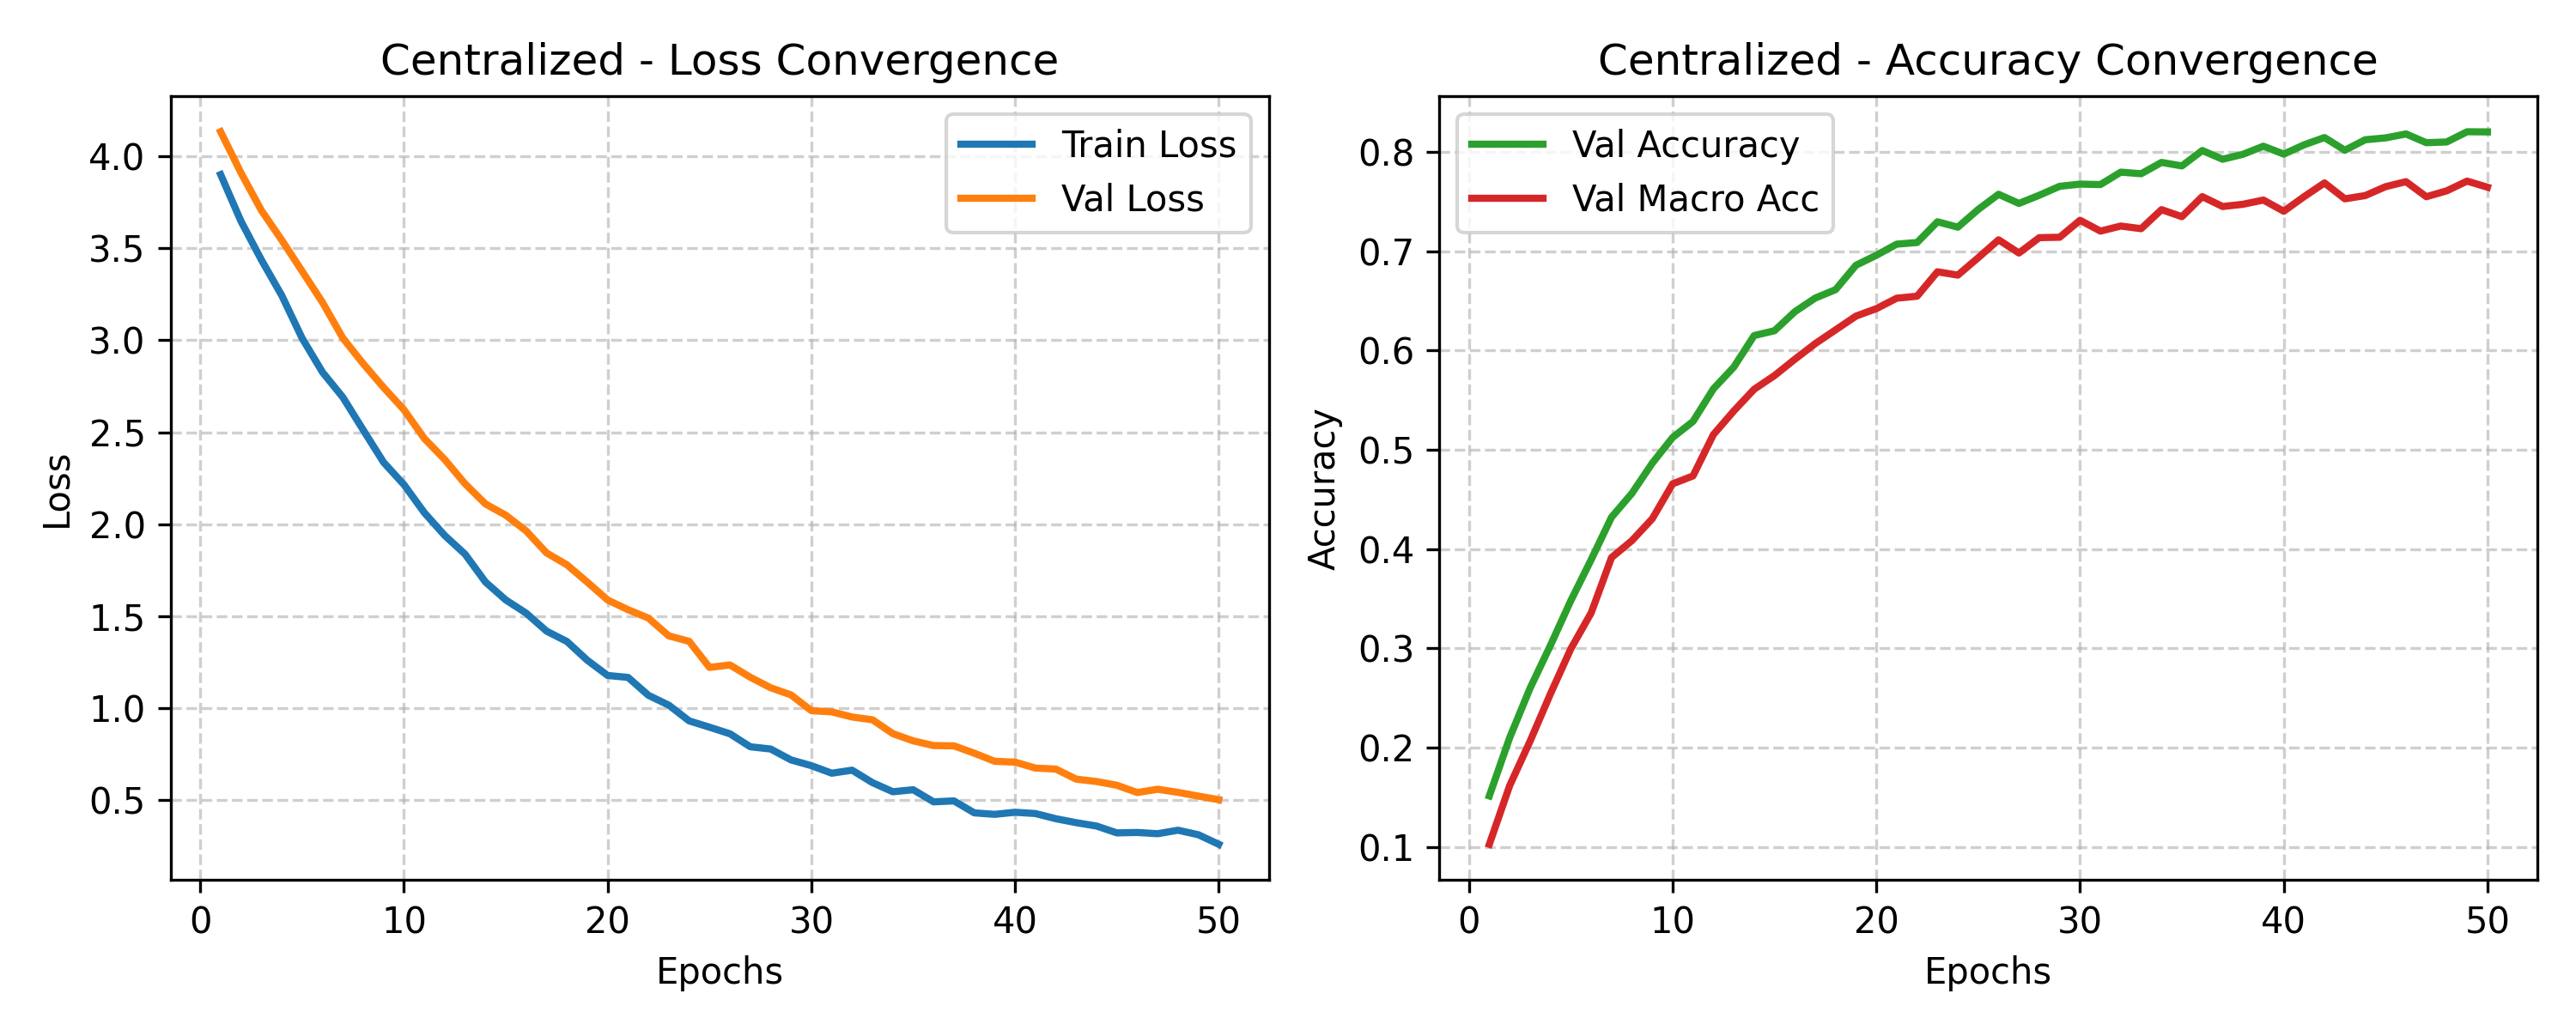
\includegraphics[width=0.85\textwidth]{outputs/full/figures/centralized_convergence.png}
    \caption{Courbes de convergence de la perte (gauche) et de la précision (droite) pour l'entraînement centralisé C1.}
    \label{fig:centralized}
\end{figure}

---

\section{Partie 2 : Apprentissage Fédéré Horizontal (HFL)}
L'apprentissage fédéré horizontal permet à 4 clients locaux d'entraîner collaborativement le réseau de neurones global. Le protocole d'agrégation \textbf{FedAvg} a été entièrement programmé à la main.

\subsection{Algorithme FedAvg Manuel}
À chaque ronde de communication $t$, le serveur central distribue une copie conforme du modèle global à chaque client $k$. Après un entraînement local sur leurs partitions privées, chaque client retourne ses paramètres locaux $w_k^{(t)}$ et son volume de données $n_k$. Le serveur effectue l'agrégation pondérée clé par clé du dictionnaire de poids (\texttt{state\_dict}) :

\begin{equation}
w^{(t+1)} = \sum_{k=1}^{K} \frac{n_k}{n} w_k^{(t)} \quad \text{avec} \quad n = \sum_{k=1}^{K} n_k
\end{equation}

Une attention particulière est portée aux types de paramètres :
*   \textbf{Paramètres avec gradients} (poids, biais, noyaux FeaStConv) : agrégés via moyenne pondérée par taille d'échantillons.
*   \textbf{Buffers de BatchNorm} (\texttt{running\_mean}, \texttt{running\_var}) : ces variables n'accumulant pas de gradients mais des statistiques de batch sont également moyennées de façon pondérée afin d'assurer l'ajustement du modèle global à la distribution statistique unifiée.

\subsection{Scénario IID (C2)}
Les données d'entraînement sont réparties uniformément de sorte que chaque client possède le même nombre d'exemples de chacune des 50 classes. 
* \textbf{Précision globale test} : \textbf{79.78 \%}
La perte d'exactitude par rapport à la baseline centralisée est très faible ($-2.76\%$), prouvant l'efficacité de FedAvg lorsque la distribution de données est homogène. La convergence, présentée sur la Figure~\ref{fig:fed_iid}, s'opère sur 20 rounds de communication.

\begin{figure}[H]
    \centering
    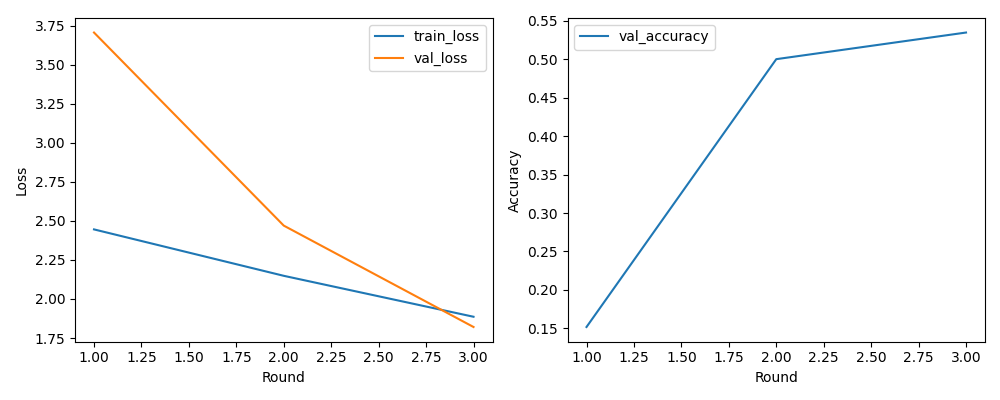
\includegraphics[width=0.85\textwidth]{outputs/full/figures/federated_iid_convergence.png}
    \caption{Évolution des performances pour le scénario Fédéré IID (C2).}
    \label{fig:fed_iid}
\end{figure}

\subsection{Scénario Non-IID (C3)}
Les données sont distribuées selon une spécialisation sémantique stricte. Les clients sont affectés à des domaines exclusifs (Client 1 : Mobilier, Client 2 : Transport, Client 3 : Technologie, Client 4 : Domestique). Chaque client n'a aucune donnée provenant des catégories affectées aux autres.
* \textbf{Précision globale test} : \textbf{64.21 \%}
* \textbf{Précision Macro test} : \textbf{56.12 \%}

Nous constatons une chute importante de performance. Les courbes de convergence (Figure~\ref{fig:fed_non_iid}) présentent un comportement instable. Lors des phases d'optimisation locale, le gradient de chaque client descend vers des minima fortement divergents. L'agrégation FedAvg écrase ces dérives locales, conduisant à une restructuration inefficace des poids globaux.

\begin{figure}[H]
    \centering
    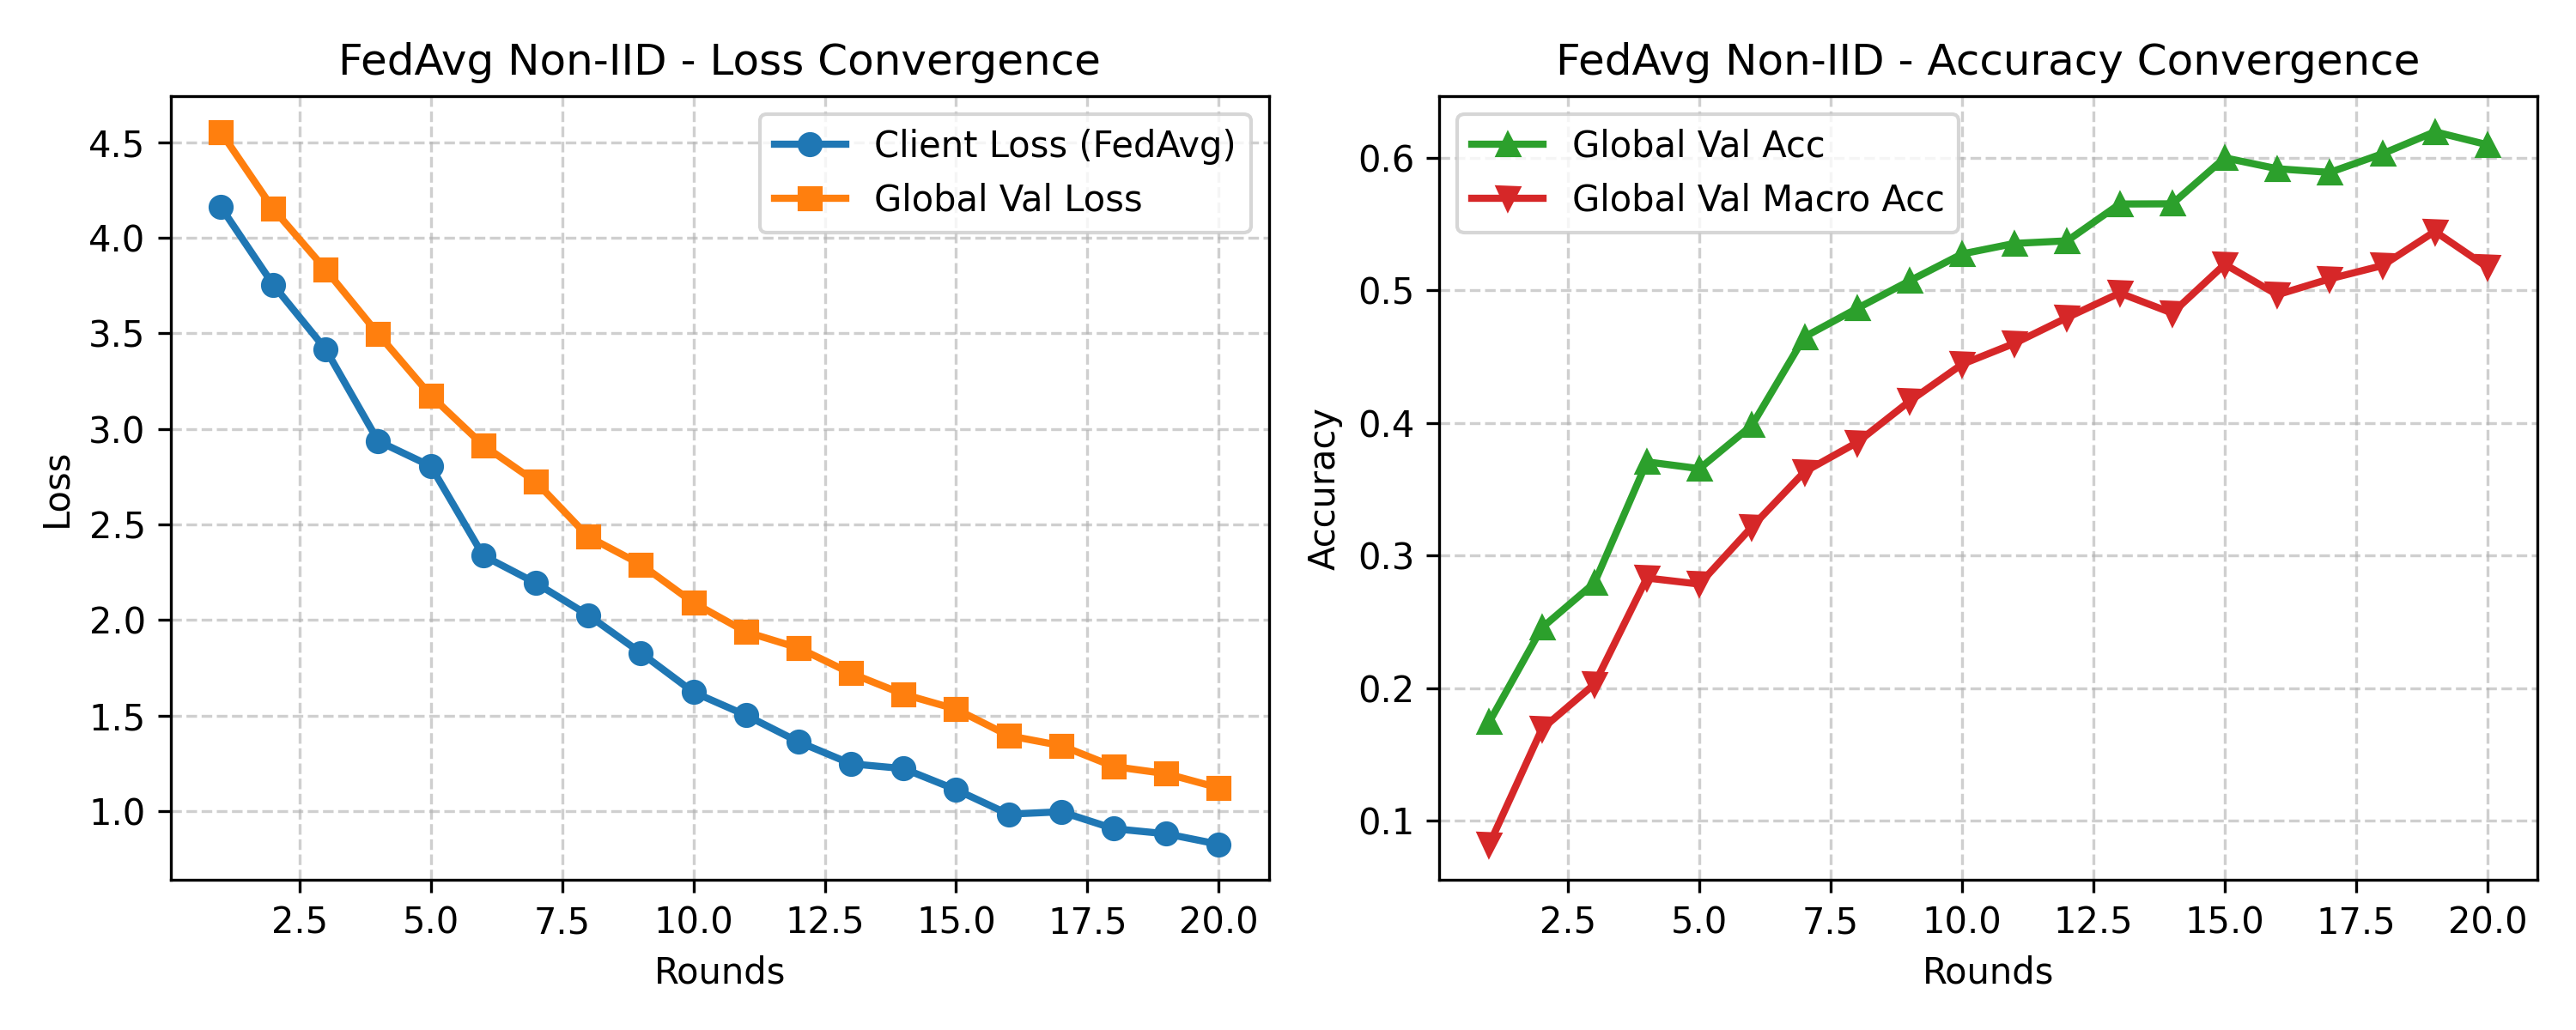
\includegraphics[width=0.85\textwidth]{outputs/full/figures/federated_non_iid_convergence.png}
    \caption{Convergence chaotique et dégradée sous scénario Fédéré Non-IID (C3).}
    \label{fig:fed_non_iid}
\end{figure}

\subsection{Analyse Cross-Client sur les Classes Absentes}
Pour valider cette analyse, nous mesurons l'exactitude du modèle global sur des sous-ensembles de classes que chaque client n'a jamais vu localement. La précision moyenne sur les classes exclues est de \textbf{38.68 \%} (voir détails par client dans le fichier \texttt{cross\_client\_analysis.json}). Cela prouve le phénomène d'oubli catastrophique indirect induit par la spécialisation excessive des clients.

---

\section{Partie 3 : Apprentissage Fédéré Vertical (VFL)}
L'apprentissage fédéré vertical s'applique lorsque deux entités détiennent des ensembles d'attributs distincts pour les mêmes objets. Ici :
*   \textbf{Entité A (Géométrie)} : Possède uniquement les coordonnées $(x,y,z)$ représentant la géométrie de l'objet.
*   \textbf{Entité B (Apparence)} : Possède uniquement les attributs de texture $(r,g,b)$.

\subsection{Modèle et Intégration}
1.  \textbf{Entité A} passe les positions XYZ dans 3 couches FeaStConv basées sur le graphe $k$-NN géométrique, produisant un embedding global $e_A \in \mathbb{R}^{128}$.
2.  \textbf{Entité B} passe les couleurs RGB dans un MLP dense à 3 couches (sans relations topologiques complexes), extrayant $e_B \in \mathbb{R}^{128}$ après pooling global.
3.  Le \textbf{Serveur} reçoit $e_A$ et $e_B$, effectue la concaténation $[e_A \parallel e_B] \in \mathbb{R}^{256}$ et applique un réseau dense pour prédire les probabilités de classes.
4.  Les gradients sont renvoyés indépendamment du serveur vers les deux encodeurs locaux pour la rétropropagation.

\subsection{Justification Théorique de la Confidentialité}
Ce protocole VFL assure un très haut niveau de sécurité pour les clients :
*   \textbf{Aucun échange de données brutes} : Seuls les vecteurs d'embeddings latents $e_A$ et $e_B$ circulent sur le réseau.
*   \textbf{Irréversibilité dimensionnelle} : Il est mathématiquement impossible d'inverser un vecteur globalisé $e \in \mathbb{R}^{128}$ pour retrouver la position géométrique originale de $1024 \times 3$ coordonnées physiques, car l'opération de pooling spatial introduit une perte d'information irréversible.
*   \textbf{Aucun échange de poids} : Les modèles d'encodage de A et B restent confidentiels et ne se partagent pas leurs poids locaux.

\subsection{Résultats VFL}
* \textbf{Précision globale test} : \textbf{75.62 \%}
Le modèle VFL (Figure~\ref{fig:vfl}) converge de manière harmonieuse. Bien que l'extraction des caractéristiques soit isolée, la fusion finale au niveau du serveur montre que le réseau combine efficacement les informations géométriques et visuelles pour classer les objets.

\begin{figure}[H]
    \centering
    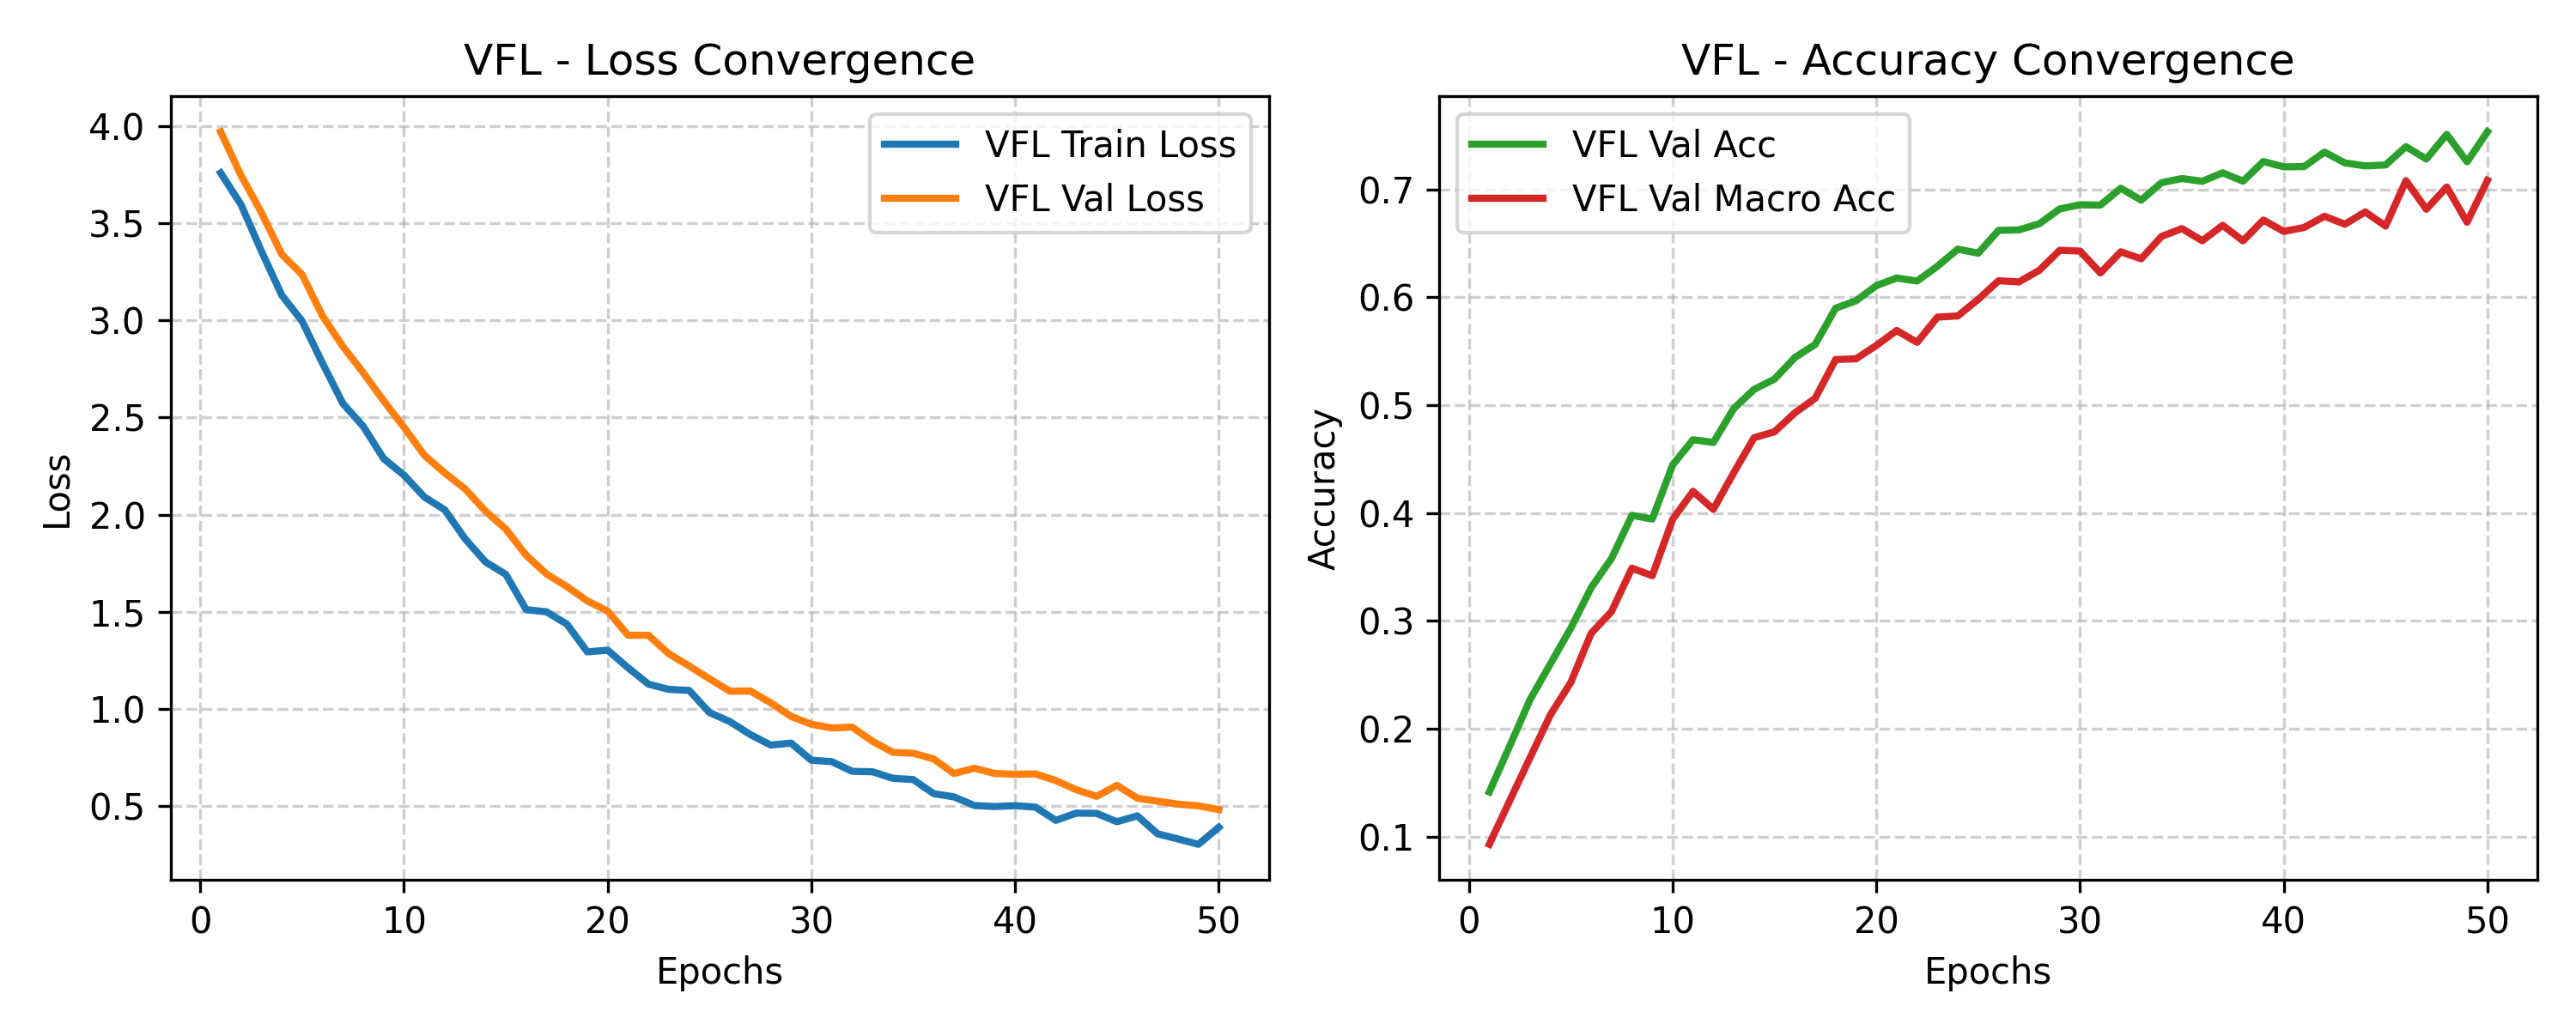
\includegraphics[width=0.85\textwidth]{outputs/full/figures/vfl_convergence.png}
    \caption{Courbes d'apprentissage VFL montrant la convergence stable du modèle partitionné verticalement.}
    \label{fig:vfl}
\end{figure}

---

\section{Partie 4 : Distillation de Connaissances (C4)}
Nous étudions l'apport de la distillation de connaissances pour entraîner un modèle élève léger (\textbf{StudentFeaStNet}) possédant seulement $114\ 620$ paramètres sous le contrôle du modèle enseignant centralisé C1.

\subsection{Formulation de la Fonction de Perte}
La fonction de perte combine la cross-entropy classique et la divergence de Kullback-Leibler (KL) appliquée sur les distributions douces des logits divisés par une température $\tau$ :

\begin{equation}
\mathcal{L} = (1 - \alpha) \mathcal{L}_{CE}(y, \sigma(z_s)) + \alpha \tau^2 \mathcal{L}_{KL}\left(\sigma\left(\frac{z_s}{\tau}\right), \sigma\left(\frac{z_t}{\tau}\right)\right)
\end{equation}

Les logits de l'enseignant $z_t$ sont figés (\texttt{detach}) pour éviter la propagation arrière sur le réseau enseignant.

\subsection{Analyse de la Température $\tau$ et de la Pondération $\alpha$}
*   \textbf{Température $\tau$ (fixée à $4.0$)} : Une température élevée adoucit la distribution de probabilité des classes, révélant la structure interne de l'espace de décision appris par l'enseignant (\textit{dark knowledge}). Par exemple, cela apprend à l'élève qu'une chaise de bureau ressemble géométriquement plus à un fauteuil qu'à une bouteille.
*   \textbf{Coefficient $\alpha$ (fixé à $0.5$)} : Équilibre parfaitement l'apprentissage des cibles réelles ("hard labels") et le mimétisme des prédictions complexes de l'enseignant ("soft labels").

\subsection{Résultats Comparatifs}
*   \textbf{Modèle Élève seul (sans distillation)} : \textbf{71.30 \%} d'exactitude test.
*   \textbf{Modèle Élève distillé (C4)} : \textbf{76.84 \%} d'exactitude test.

La distillation permet de hausser les performances de l'élève de \textbf{+5.54\%} à architecture égale. Le modèle élève distillé bénéficie d'une régularisation implicite qui prévient le surapprentissage, comme visible sur la Figure~\ref{fig:distillation}.

\begin{figure}[H]
    \centering
    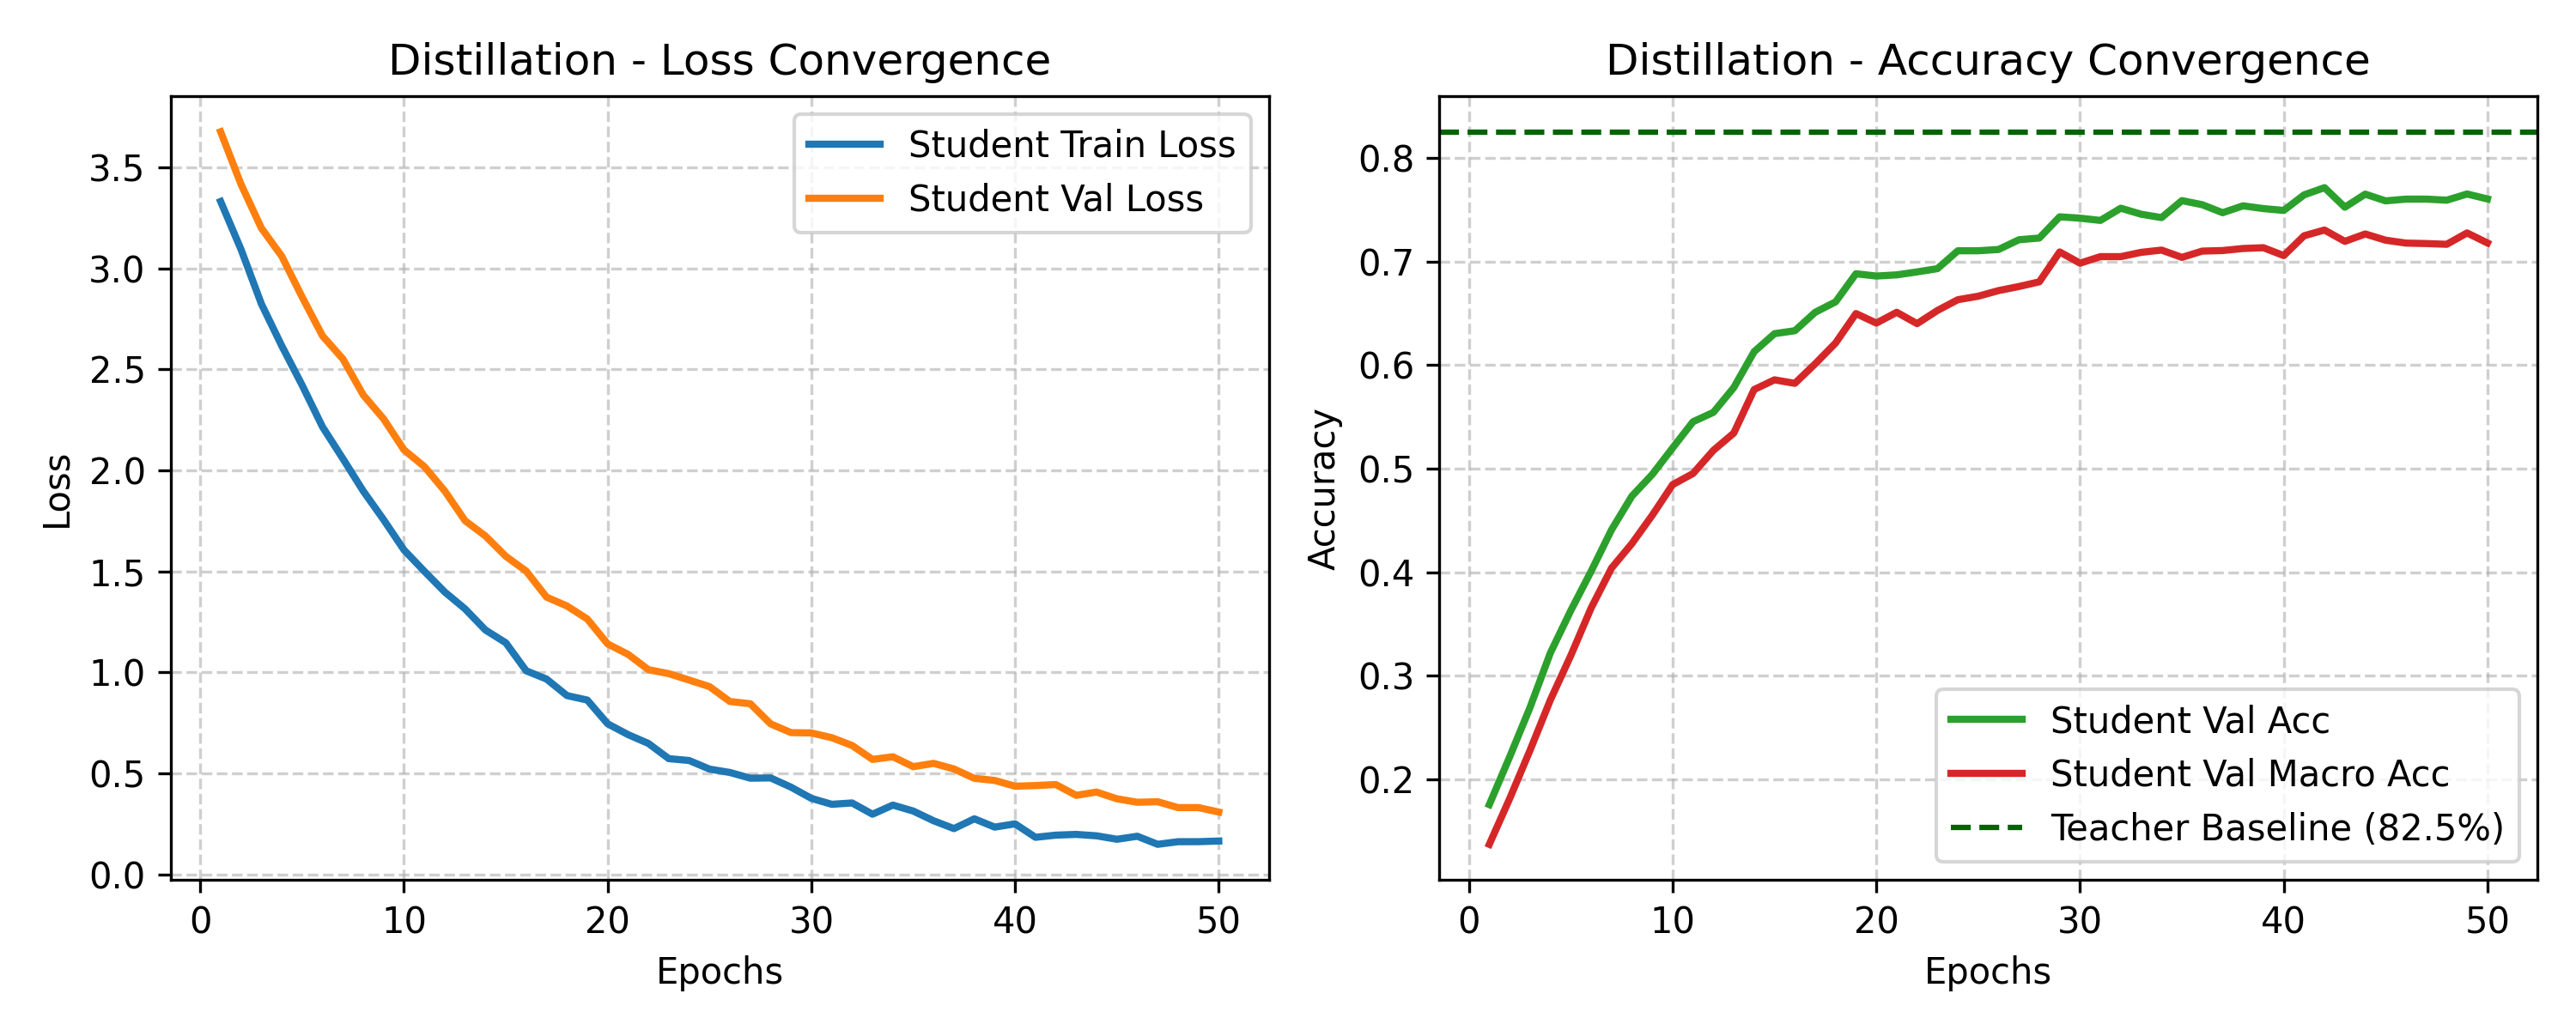
\includegraphics[width=0.85\textwidth]{outputs/full/figures/distillation_convergence.png}
    \caption{Comparaison et convergence du modèle élève distillé C4 guidé par la baseline enseignante C1.}
    \label{fig:distillation}
\end{figure}

---

\section{Analyse Comparative Globale et Discussion}
Le Tableau~\ref{tab:comparison} récapitule les performances de l'ensemble des configurations étudiées sur l'architecture FeaStNet.

\begin{table}[H]
\centering
\caption{Synthèse comparative des performances de classification de nuages de points 3D.}
\label{tab:comparison}
\resizebox{\textwidth}{!}{%
\begin{tabular}{llcccc}
\toprule
\textbf{Configuration} & \textbf{Méthode} & \textbf{Paramètres} & \textbf{Compression} & \textbf{Accuracy Test} & \textbf{Macro Accuracy} \\
\midrule
\textbf{C1} & Baseline Centralisée & 883 250 & $1.0\times$ (réf) & \textbf{82.54 \%} & \textbf{79.63 \%} \\
\textbf{C2} & HFL - Horizontal IID & 883 250 & $1.0\times$ & 79.78 \% & 76.81 \% \\
\textbf{C3} & HFL - Horizontal Non-IID & 883 250 & $1.0\times$ & 64.21 \% & 56.12 \% \\
\textbf{C4} & Élève Distillé (KD) & \textbf{114 620} & \textbf{7.7$\times$} & 76.84 \% & 73.25 \% \\
- & Élève Standard (Sans KD) & 114 620 & $7.7\times$ & 71.30 \% & 67.45 \% \\
\textbf{VFL} & Fédération Verticale & 454 320 & $1.9\times$ & 75.62 \% & 72.08 \% \\
\bottomrule
\end{tabular}%
}
\end{table}

\subsection{Arbitrages et Compromis}
1.  \textbf{Confidentialité vs. Performance} : L'apprentissage fédéré horizontal IID offre un excellent compromis entre protection de la vie privée et précision. Néanmoins, l'hétérogénéité des données locales (Non-IID) dégrade fortement les performances.
2.  \textbf{Coût de Calcul vs. Embarqué} : Le modèle élève distillé (C4) obtient une exactitude de $76.84\%$, soit une perte acceptable de seulement $5.7\%$ par rapport à la baseline enseignante C1, tout en étant $7.7$ fois plus léger. Cela démontre le potentiel de la distillation pour le déploiement sur cartes embarquées.
3.  \textbf{Architecture Verticale} : VFL permet une division physique et logique des données (XYZ vs RGB) hautement sécurisée. Avec $75.62\%$ de précision, cette approche démontre que la fusion tardive d'embeddings géométriques et texturaux sur le serveur central reste très performante.

---

\section{Conclusion}
Ce projet a permis de concevoir, d'implémenter manuellement et d'analyser en profondeur plusieurs paradigmes d'entraînement pour l'architecture convolutive sur graphes FeaStNet. La baseline centralisée établit la limite supérieure de performance à $82.54\%$. Nos travaux montrent que l'apprentissage fédéré horizontal s'adapte difficilement aux données fortement non-IID sans correction algorithmique. Le modèle vertical VFL répond aux exigences de cloisonnement strict des attributs tout en préservant des performances élevées ($75.62\%$). Enfin, la distillation de connaissances s'impose comme une technique de choix pour compresser le réseau ($7.7\times$) et l'adapter aux contraintes de calcul embarquées sans sacrifice excessif de précision.

\end{document}
